\section{Vybrané integrované obvody}

\begin{table}[H]
	\begin{center}

		\begin{tabular}{cc}
			\begin{minipage}{0.5\textwidth}
				\begin{figure}[H]
					\centering
					\includegraphics[height=5.9cm]{img/LM25085.pdf}
					\caption{Blokové schéma LM25085}
					\label{graf:1}
				\end{figure}
			\end{minipage}

	&		
				
			\begin{minipage}{0.5\textwidth}
				\begin{figure}[H]
					\centering
					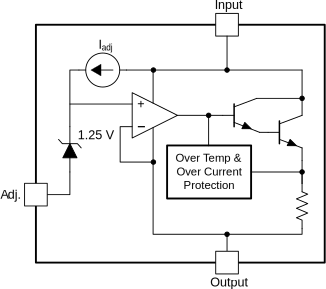
\includegraphics[height=5.9cm]{img/LM317.pdf}
					\caption{Blokové schéma LM317}
					\label{graf:1}
				\end{figure}
			\end{minipage}
		\end{tabular}
	\end{center}	
\end{table}

LM25085 je regulátor PFET tranzistorů učený do spínaných snižujících měničů s vysokou účinností (buck). Naproti tomu LM317 je notoricky známý integrovaný obvod určený především jako lineární stabilizátor napětí, popřípadě drobnou úpravou okolních součástek a zapojení jako zdroj stabilního proudu.